\lab{The Finite Difference Method}{The Finite Difference Method}
\label{lab:finitedifference2}

Suppose we have a function $u(x)$, defined on an interval $[a,b]$.
Let $a = x_{-1}, x_0, x_1, \ldots x_{n-1}$ be a grid of evenly spaced points, with $x_i = a + (i+1)h$, $h = (b-a)/n$.
From a Taylor expansion of $u(x)$, we obtain the approximation
\[u''(x) = \frac{u(x+h) - 2u(x) + u(x-h)}{h^2}, \]
with error $E(h) = \mathcal{O}(h^2)$.
Thus
\[u''(x) = \frac{u(x_{i+1}) - 2u(x_i) + u(x_{i-1})}{h^2}, \quad i = 0, \ldots, n-2.\]
This can be written in matrix form as
\begin{align}
\frac{1}{h^2}
\begin{bmatrix}
-2 & 1 & \\
1 & -2 & 1  \\
& &\ddots & \\
 & 1 & -2 & 1 \\
 & & 1 & -2
\end{bmatrix}
\begin{bmatrix}
u(x_0) \\ u(x_1)\\ \vdots  \\ u(x_{n-3}) \\ u(x_{n-2})
\end{bmatrix} +
\begin{bmatrix}
u(x_{-1})/h^2 \\ 0 \\ \vdots  \\ 0 \\ u(x_{n-1})/h^2
\end{bmatrix} =
\begin{bmatrix}
u''(x_0) \\ u''(x_1)\\ \vdots  \\ u''(x_{n-3}) \\ u''(x_{n-2})
\end{bmatrix}\label{finitedifference2:upp}
\end{align}

Similarly, since  $u'(x) = (u(x+h) - u(x-h))/(2h)$ with error $E(h) = \mathcal{O}(h^2)$, we have the approximation
\begin{align}
\frac{1}{2h}
\begin{bmatrix}
0 & 1 & \\
-1 & 0 & 1  \\
& &\ddots & \\
 & -1 & 0 & 1 \\
 & & -1 & 0
\end{bmatrix}
\begin{bmatrix}
u(x_0) \\ u(x_1)\\ \vdots  \\ u(x_{n-3}) \\ u(x_{n-2})
\end{bmatrix} +
\begin{bmatrix}
-u(x_{-1})/(2h) \\ 0 \\ \vdots  \\ 0 \\ u(x_{n-1})/(2h)
\end{bmatrix} =
\begin{bmatrix}
u'(x_0) \\ u'(x_1)\\ \vdots  \\ u'(x_{n-3}) \\ u'(x_{n-2})
\end{bmatrix}\label{finitedifference2:up}
\end{align}

\begin{problem}
	Use \eqref{finitedifference2:upp} and \eqref{finitedifference2:up} to approximate $\frac{1}{2}u'' - u$ at the grid points.
\end{problem}

Suppose that instead of knowing the function $u(x)$, we know that $\frac{1}{2}u'' - u = f$, where the function $f(x)$ is given.
How do we solve for $u$ at the grid points?

\section*{Finite Difference Methods}

Numerical methods for differential equations seek to approximate the exact solution $u(x)$ at some finite collection of points in the domain of the problem.
Instead of analytically solving the original differential equation, defined over an infinite-dimensional function space, they use a simple finite collection of algebraic equations to approximate the original problem.

Consider the following differential equation:
\begin{align}
	\begin{split}
	&{ } \epsilon u''(x)-u'= f(x), \quad x \in (0,1), \\
	&{ } u(0) = 1, \quad u(1) = 3.
	\end{split} \label{eqn:singular_perturbed_BVP}
\end{align}
Equation\eqref{eqn:singular_perturbed_BVP} can be written $D u = f,$ where $D = \epsilon \frac{d^2}{dx^2} - \frac{d}{dx}$ is a differential operator defined on the infinite-dimensional space of functions $u:[0,1] \to \mathbb{R}$ that are twice continuously differentiable and satisfy the boundary conditions $u(0) = 1$, $u(1) = 3$.

We look for an approximate solution $\{U_i\}_{i=-1}^N$ on an evenly spaced grid of $N$ subintervals, $a = x_{-1}, x_0, \ldots, x_{N-1} = b$ with $h = x_{i+1}-x_i$ for each $i$.
Our finite difference method will replace the differential operator $D = \epsilon \frac{d^2}{dx^2} - \frac{d}{dx}$, defined on an infinite-dimensional space of functions, with difference operators defined on a finite vector space (i.e., the space of grid functions $\{U_i\}_{i=-1}^N$).
To do this, we replace derivative terms in the differential equation with appropriate difference expressions.

Recalling that
\begin{align*}
	\frac{d^2}{dx^2} u(x) &= \frac{u(x+h)- 2u(x) + u(x-h)}{h^2} + \mathcal{O}(h^2),\\
\frac{d}{dx} u(x) &= \frac{u(x+h)-u(x-h)}{2h} + \mathcal{O}(h^2).
\end{align*}
we define the finite difference operator $D_h$ by
\[
D_h U_i = \epsilon \frac{1}{h^2}\left(U_{i+1} -2U_i + U_{i-1}\right) - \frac{1}{2h} \left(U_{i+1}-U_{i-1} \right).
\]
Thus we discretize equation \eqref{eqn:singular_perturbed_BVP} using the equations
\begin{align*}
	\frac{\epsilon}{h^2} (U_{i+1}- 2U_i + U_{i-1}) - \frac{1}{2h} \left(U_{i+1}-U_{i-1} \right)  &= f(x_i), \quad i = 0, \ldots, N-2,
\end{align*}
along with boundary conditions $U_{-1} = 1,$ $U_{N-1} = 3$.

This gives $N+1$ equations and $N+1$ unknowns, and can be written in matrix form as
\[ \frac{1}{h^2} \begin{bmatrix}h^2 & 0 &0&\hdots &0 \\ (\epsilon + h/2) &-2\epsilon & (\epsilon - h/2) &\hdots &0\\ \vdots &  & \ddots & &\vdots \\
0 & \hdots & (\epsilon + h/2) &-2\epsilon & (\epsilon - h/2) \\ 0 & \hdots & & 0 & h^2
\end{bmatrix} \cdot \begin{bmatrix}U_{-1}\\U_0\\ \vdots \\U_{N-2} \\U_{N-1}\end{bmatrix} = \begin{bmatrix}f(x_{-1})\\f(x_0)\\ \vdots \\ f(x_{N-2}) \\ f(x_{N-1}) \end{bmatrix}.
\]
We can further modify the system to obtain an $(N-1)\times (N-1)$ tridiagonal matrix on the left:
\[\frac{1}{h^2} \begin{bmatrix}-2\epsilon & (\epsilon - h/2) &0&\hdots &0 \\ (\epsilon + h/2) &-2\epsilon & (\epsilon - h/2) &\hdots &0\\ \vdots &  & \ddots & &\vdots \\
0 & \hdots & (\epsilon + h/2) &-2\epsilon & (\epsilon - h/2) \\ 0 & \hdots & & (\epsilon + h/2) &-2\epsilon
\end{bmatrix} \cdot \begin{bmatrix}U_{0}\\U_1\\ \vdots \\U_{N-3} \\U_{N-2}\end{bmatrix} = \begin{bmatrix}f(x_0) -\alpha(\epsilon + h/2)/h^2 \\f(x_1)\\ \vdots \\ f(x_{N-3})\\ f(x_{N-2})-\beta(\epsilon - h/2)/h^2 \end{bmatrix}.
\]

\begin{comment}
\begin{lstlisting}
import numpy as np
from scipy.sparse import spdiags
from scipy.sparse.linalg import spsolve
import matplotlib.pyplot as plt

def bvp(func, epsilon, alpha, beta, N):
	a,b = 0., 1. 	# Interval for the BVP
	h = (b-a)/N 	# The length of each subinterval
	
	# Initialize and define the vector F on the right
	F = np.empty(N-1.)			
	F[0] = func(a+1.*h)-alpha*(epsilon+h/2.)*h**(-2.)
	F[N-2] = func(a+(N-1)*h)-beta*(epsilon-h/2.)*h**(-2.)
	for j in xrange(1,N-2):
		F[j] = func(a + (j+1)*h)
		
	# Here we define the arrays that will go on the diagonals of A
	data = np.empty((3,N-1))
	data[0,:] = -2.*epsilon*np.ones((1,N-1)) # main diagonal
	data[1,:]  = (epsilon+h/2.)*np.ones((1,N-1))  	 # off-diagonals
	data[2,:] = (epsilon-h/2.)*np.ones((1,N-1))
	# Next we specify on which diagonals they will be placed, and create A
	diags = np.array([0,-1,1])
	A=h**(-2.)*spdiags(data,diags,N-1,N-1).asformat('csr')
	
	U = np.empty(N+1)
	U[1:-1] = spsolve(A,F)
	U[0], U[-1] = alpha, beta
	return np.linspace(a,b,N+1), U

x, y = bvp(lambda x:-1., epsilon=.05,alpha=1, beta=3, N=400)
plt.plot(x,y,'-k',linewidth=2.0)
plt.show()

\end{lstlisting}
\end{comment}

\section*{A heuristic test for convergence}
The finite differences used above are second order approximations of the first and second derivatives of a function.  It seems reasonable to expect that the numerical solution would converge at a rate of about $\mathcal{O}(h^2)$. How can we check that a numerical approximation is reasonable?

% One way to determine this is to compute solutions for various step sizes $h$ and see if the solutions are converging to something.
Suppose a finite difference method is $\mathcal{O}(h^p)$ accurate.
This means that the error $E(h) \approx Ch^p$ for some constant $C$ as $h \to 0$ (in other words, for $h>0$ small enough).

So compute the approximation $y_k$ for each step size $h_k$, $h_1 > h_2> \ldots>h_m$.
$y_m$ should be the most accurate approximation, and will be thought of as the true solution.
Then the error of the approximation for
step size $h_k, k < m,$ is
\begin{align*}
	E(h_k) &= \max( \abs{ y_k - y_m}) \approx C h_k^p ,\\
	\log(E(h_k)) &= \log(C) + p \log(h_k).
\end{align*}
Thus on a log-log plot of $E(h)$ vs. $h$, these values should be on a straight line with slope $p$ when $h$ is small enough to start getting convergence.

The following code generates the log-log plot in Figure \ref{fig:finitedifference2}, and demonstrates second-order convergence for our finite difference approximation.
\begin{lstlisting}
num_approx = 10 # Number of Approximations
N = 5*np.array([2**j for j in range(num_approx)])
h, max_error = (1.-0)/N[:-1], np.ones(num_approx-1)

# Best numerical solution, used to approximate the true solution.
mesh_best, num_sol_best = bvp(lambda x:-1, epsilon=.1, alpha=1, beta=3, N=N[-1])
for j in range(len(N)-1):
    mesh, num_sol = bvp(lambda x:-1, epsilon=.1, alpha=1, beta=3, N=N[j])
    max_error[j] = np.max(np.abs( num_sol- num_sol_best[::2**(num_approx-j-1)] ) )
plt.loglog(h,max_error,'.-r',label="$E(h)$")
plt.loglog(h,h**(2.),'-k',label="$h^{\, 2}$")
plt.xlabel("$h$")
plt.legend(loc='best')
plt.show()
print "The order of the finite difference approximation is about ", ( (np.log(max_error[0]) -
    np.log(max_error[-1]) )/( np.log(h[0]) - np.log(h[-1]) ) ), "."
\end{lstlisting}

\begin{figure}[ht]
\centering
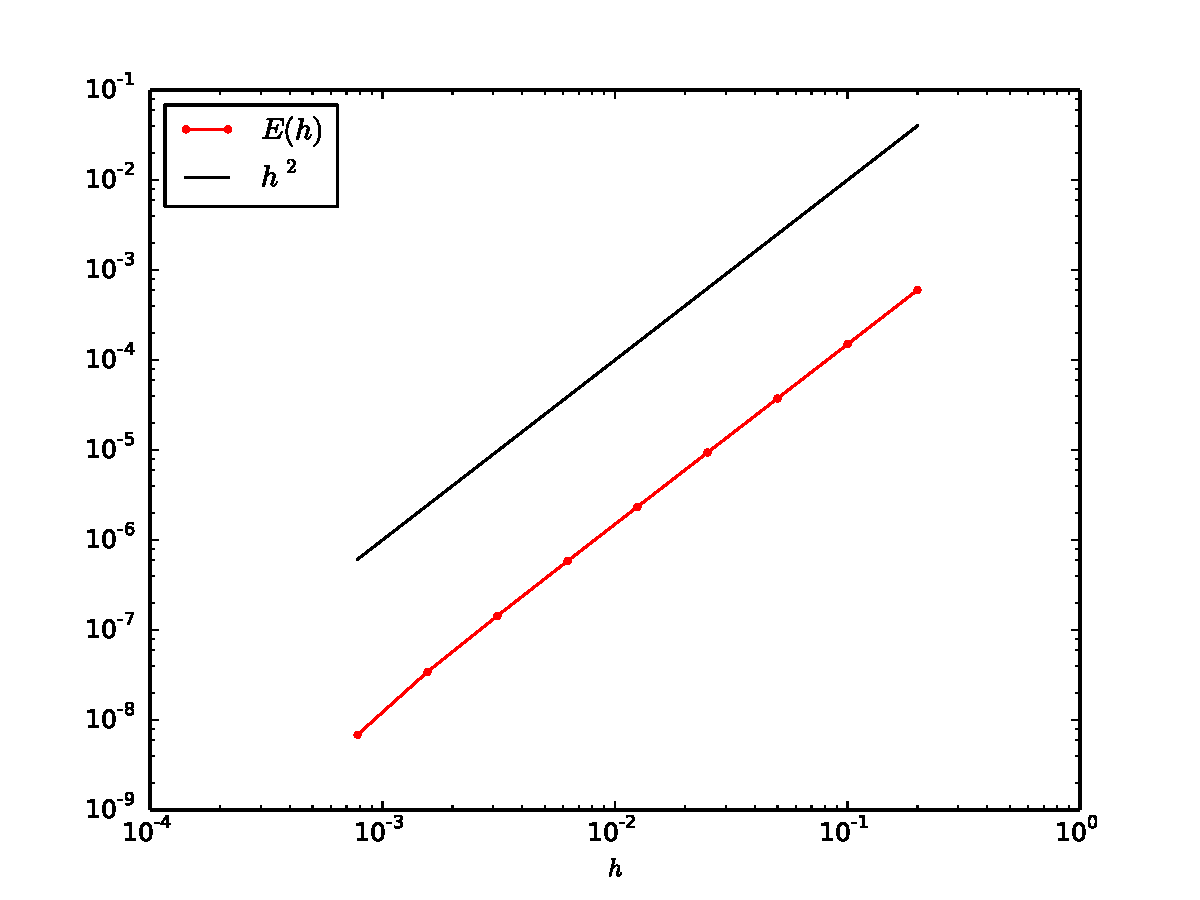
\includegraphics[width=12cm]{example_convergence.pdf}
\caption{Demonstration of second order convergence for the finite difference approximation.} \label{fig:finitedifference2}
\end{figure}

\begin{problem}
Solve the singularly perturbed BVP \eqref{eqn:singular_perturbed_BVP} with $\epsilon = 1/10$, $f(x) = -1$.
This BVP is called singularly perturbed because of the location of the parameter $\epsilon$.
For $\epsilon = 0$ the ODE has a drastically different character - it then becomes first order, and can no longer support two boundary conditions.
	
How many subintervals are needed to obtain 4 digits of accuracy?
	% If $\alpha = 1$,  $\beta = 3$, and $f(x) = -1$, there is an exact solution:
	% \[y(x) = \alpha + x+ (\beta - \alpha -1)\frac{e^{x/\epsilon -1}}{e^{1/\epsilon -1}}\]
	\label{prob:finitedifference2:prob1}
\end{problem}



\begin{problem}
Extend the given finite difference code to the case of a general second order linear BVP with Dirichlet conditions:
\begin{align*}
	&{ } a_1(x)y'' +a_2(x)y'+ a_3(x) y = f(x), \quad x \in (a,b),\\
	&{ } y(a) = \alpha, \quad y(b) = \beta.
\end{align*}
Use your code to solve the boundary value problem
\begin{align*}
	\epsilon y'' - 4(\pi - x^2)y = \cos x, \\
	y(0) = 0, \quad y(\pi/2) = 1,
\end{align*}
for $\epsilon = 0.1$.
\label{prob:finitedifference2:prob2}
\end{problem}

\begin{figure}
\centering
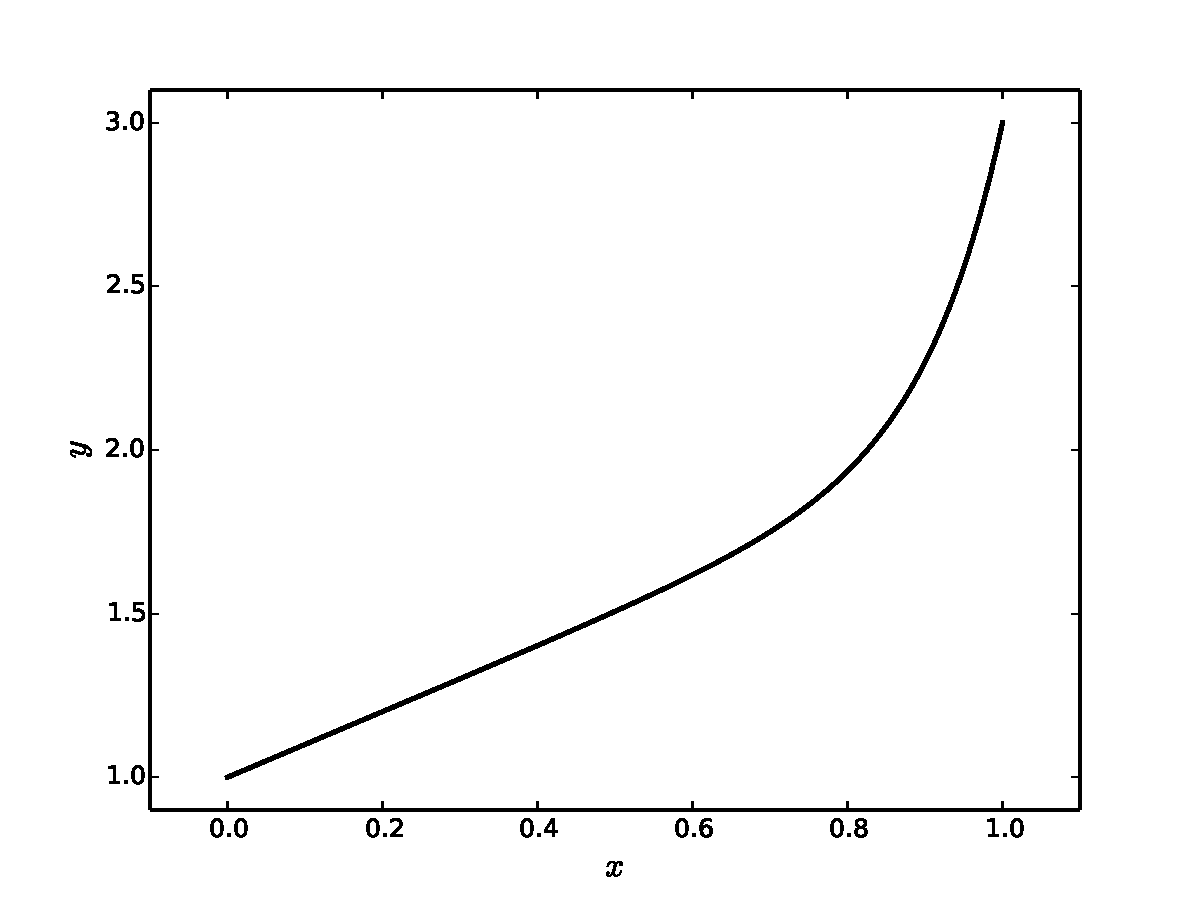
\includegraphics[width=12cm]{figure2.pdf}
\caption{The solution to Problem \ref{prob:finitedifference2:prob1}.
The solution gets steeper near $x = 1$ as $\epsilon $ gets small.}
\end{figure}

\begin{figure}
\centering
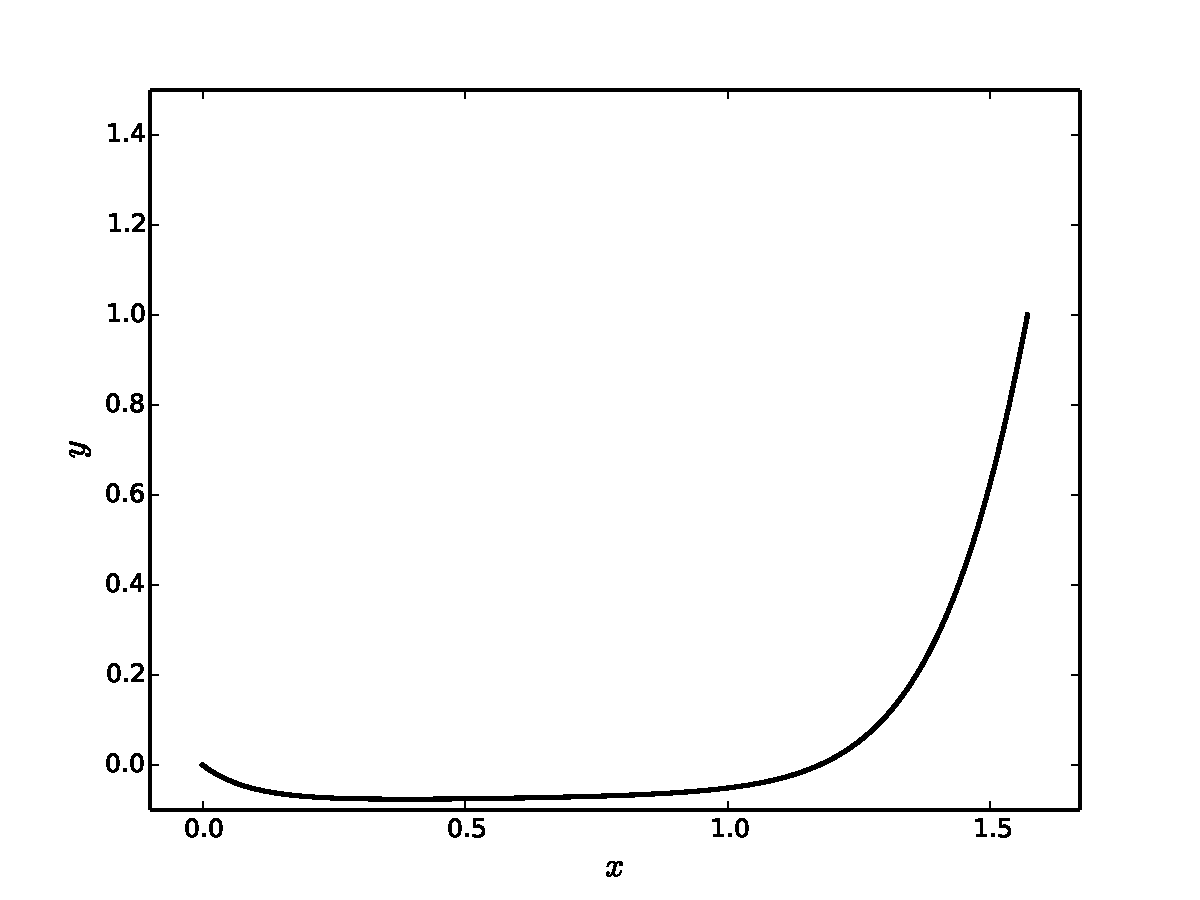
\includegraphics[width=12cm]{figure3.pdf}
\caption{The solution to Problem \ref{prob:finitedifference2:prob2}.
% The solution gets steeper near $x = 1$ as $\epsilon $ gets small.
}
\end{figure}

